\subsection{6.3 问题三：相关性与替代/互补性下的最优种植策略}
在问题二的基础上，问题三进一步考虑了\textbf{农作物之间的相关性}以及\textbf{替代性/互补性}，并将其引入到多情景风险优化模型中。为此，构建了销量（D）、价格（P）、成本（C）三类变量的相关矩阵，通过 Copula 方法生成相关随机情景,突破独立情景假设，并结合交叉价格弹性系数，对需求进行价格联动修正，最后在相同农艺与管理约束下使用遗传算法（GA）进行求解,输出优化方案、Spearman 相关系数热力图、风险 - 收益对比表，验证模型对市场联动的刻画能力，实现风险与收益的更优平衡。
\begin{figure}[H]
    \centering
    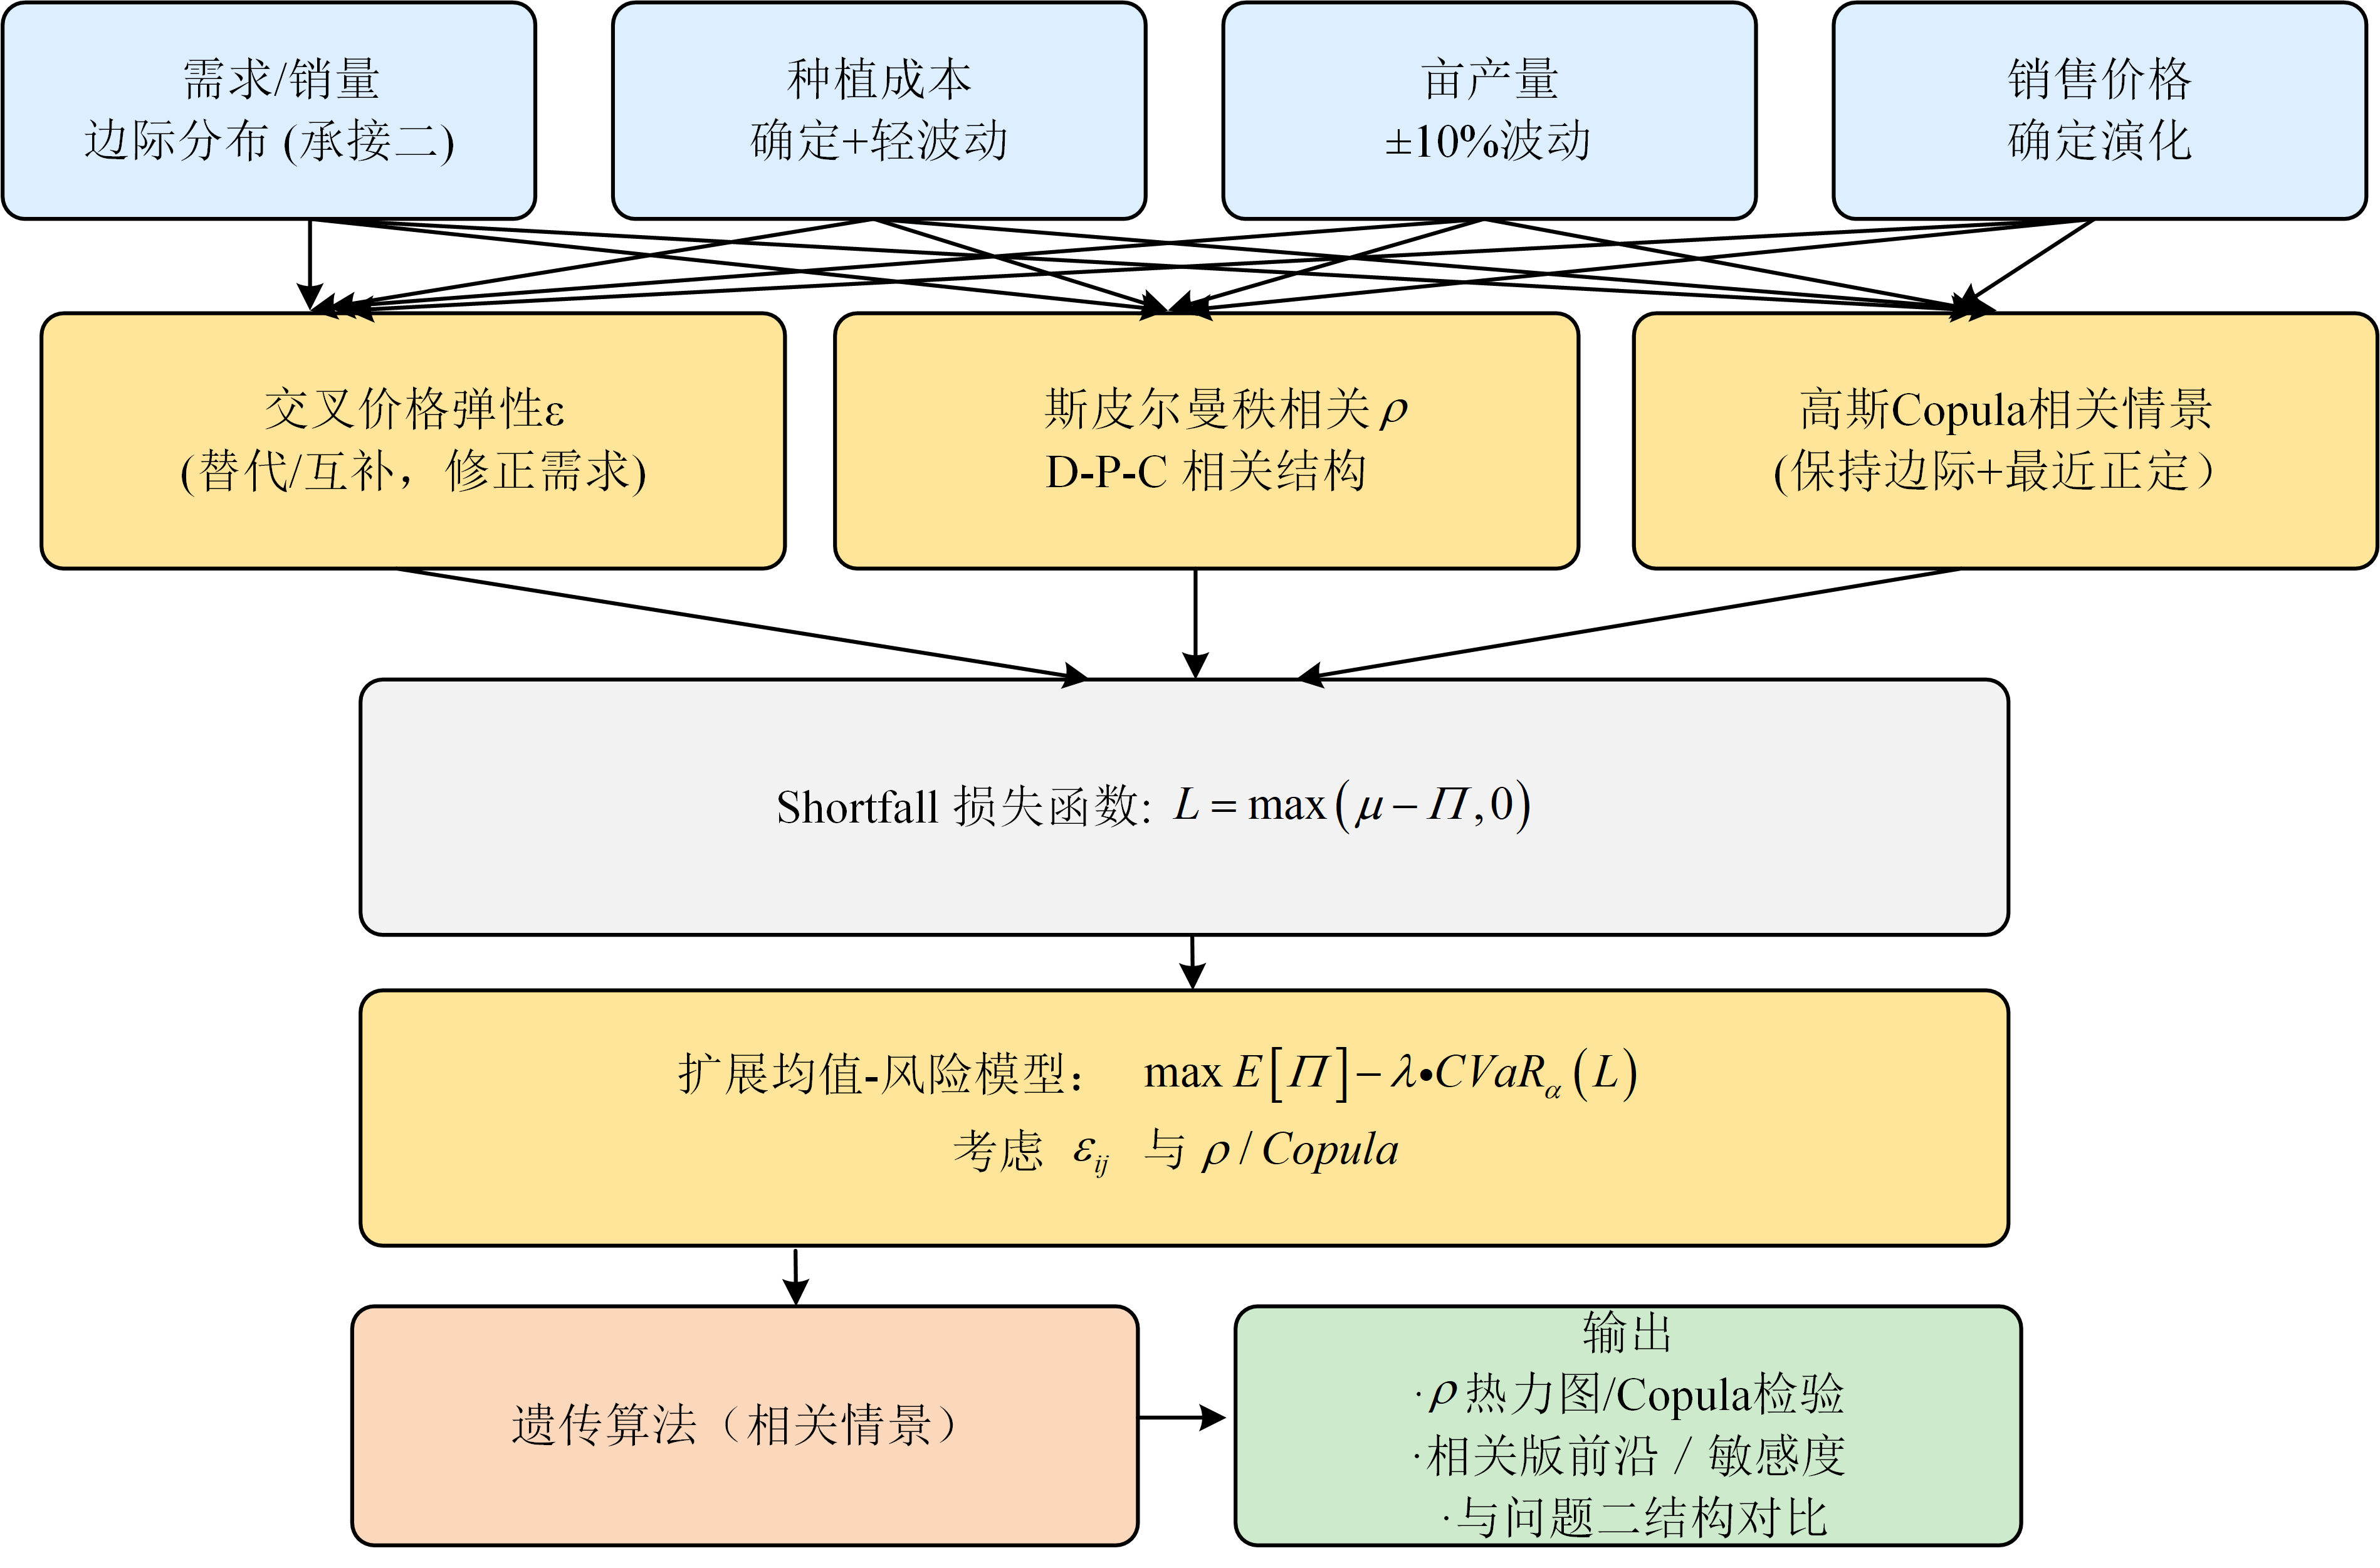
\includegraphics[width=0.8\textwidth]{mindmap/pb3.png} % 耕地类型占比图
    \caption{问题三求解流程图}
    \label{fig:mmp_pb3}
\end{figure}
\subsection{6.3.1 相关结构建模}
\textbf{Spearman-$\rho$ 热力图验证}
首先利用历史或设定的相关系数矩阵，构建了 $3C\times 3C$ 的相关性结构（$C$ 为作物数），变量顺序为 D $\rightarrow$ P $\rightarrow$ C。通过 Copula 采样生成情景后，计算 Spearman-$\rho$ 系数矩阵，并绘制热力图（图~\ref{fig:spearman_heat}），可见同类变量块之间的相关性模式与设定一致：D--P 为负相关、P--C 为正相关、同类作物价格高度相关。

\begin{figure}[htbp]
  \centering
  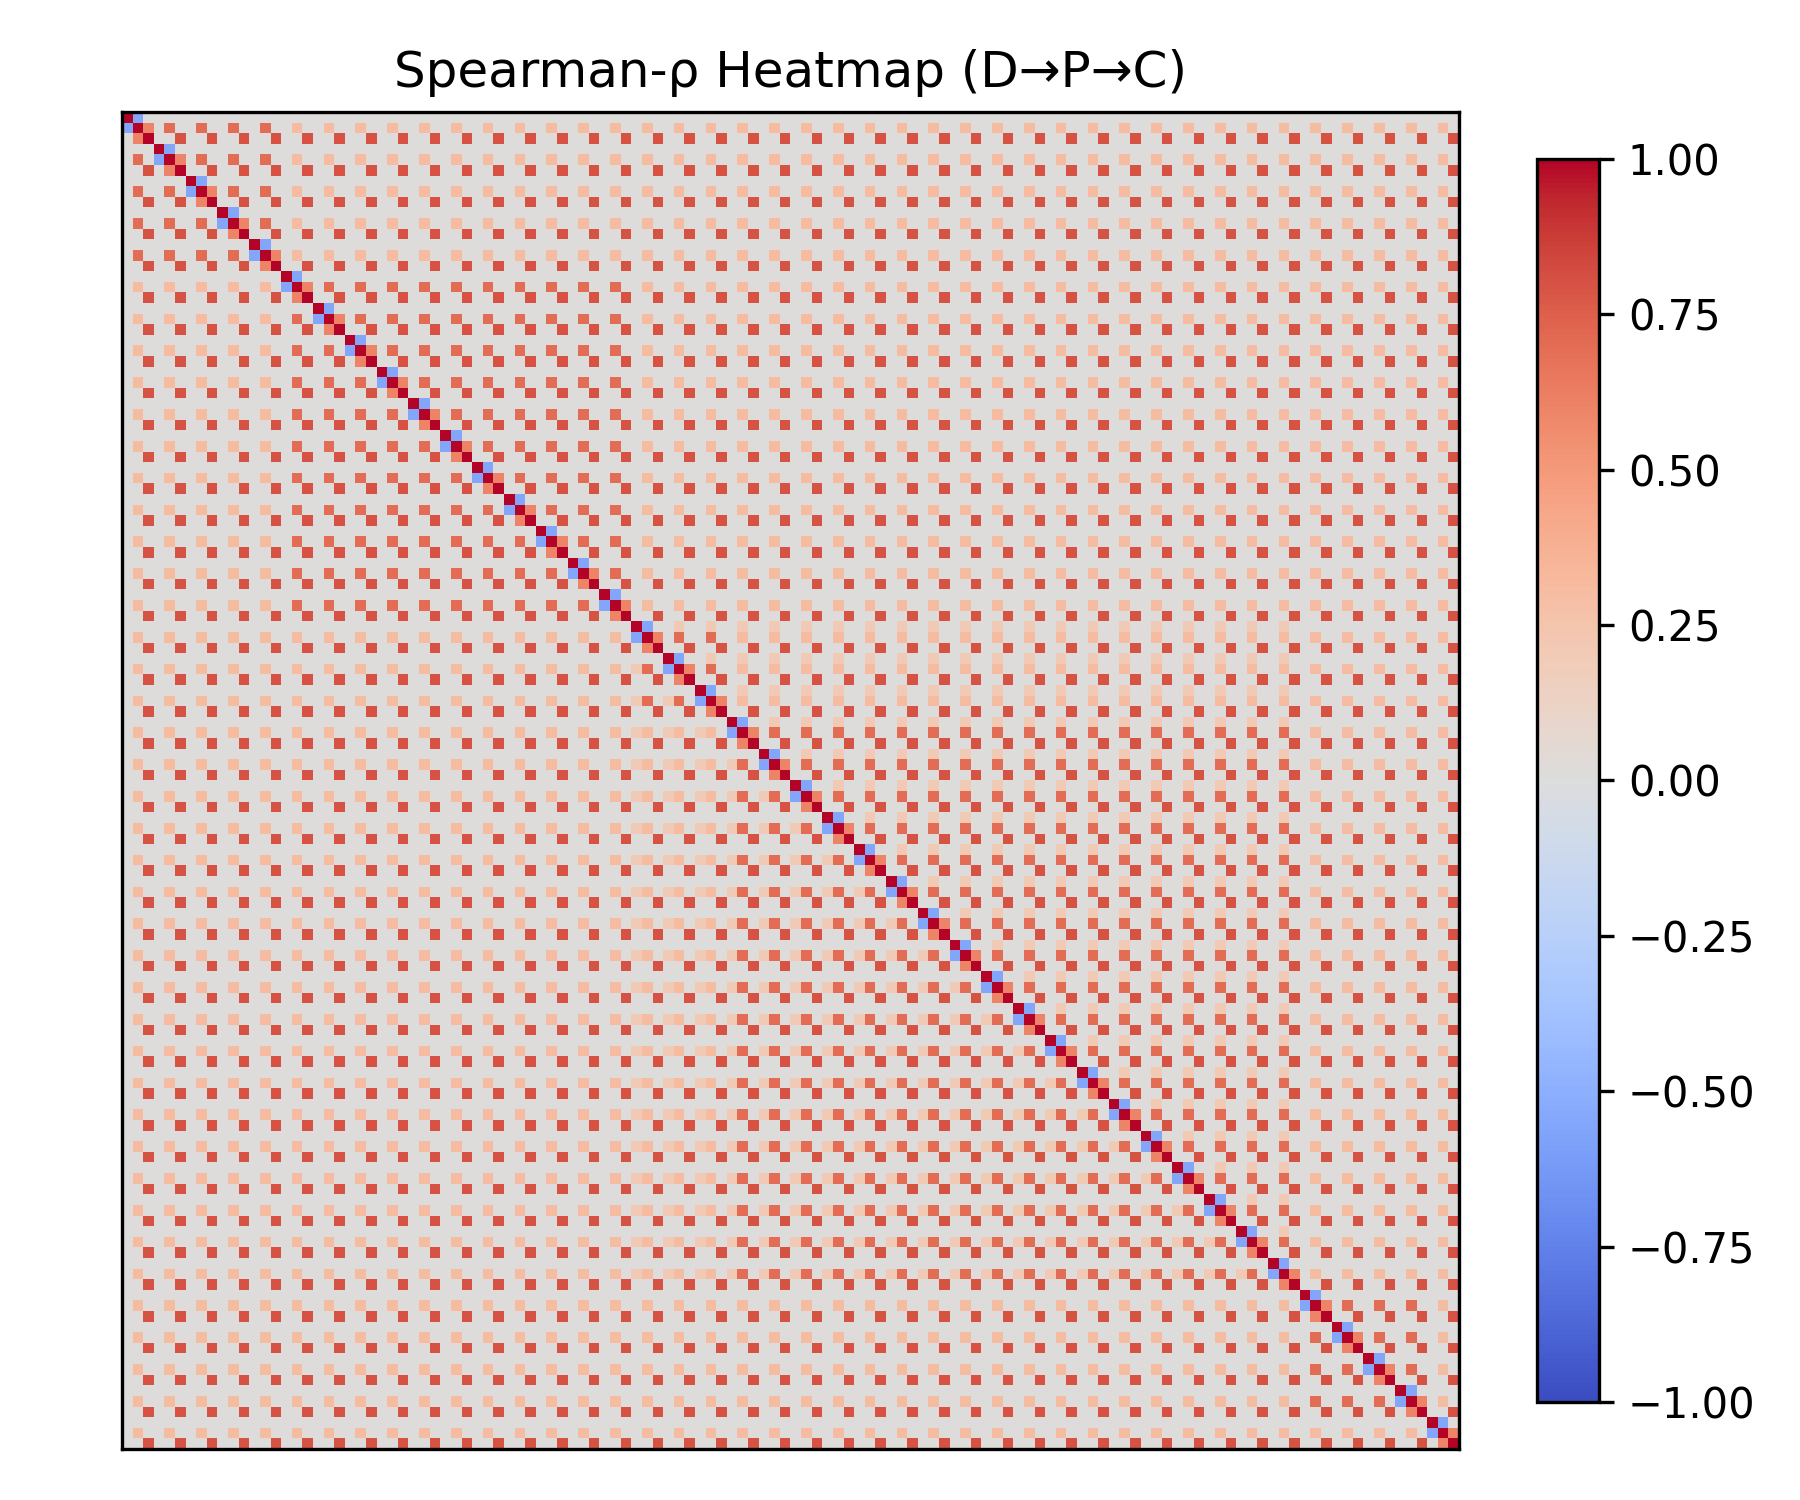
\includegraphics[width=0.86\linewidth]{figure_pb3/d6b01d20396794b667c82f8a2af2b5b5.png}
  \caption{Spearman-$\rho$ 热力图（$D\!\to\!P\!\to\!C$ 顺序）}
  \label{fig:spearman_heat}
\end{figure}

\textbf{单作物块相关性}
图~\ref{fig:triple_block} 展示了示例作物的 D--P--C 三变量相关系数块（秩相关）。\begin{figure}[htbp]
  \centering
  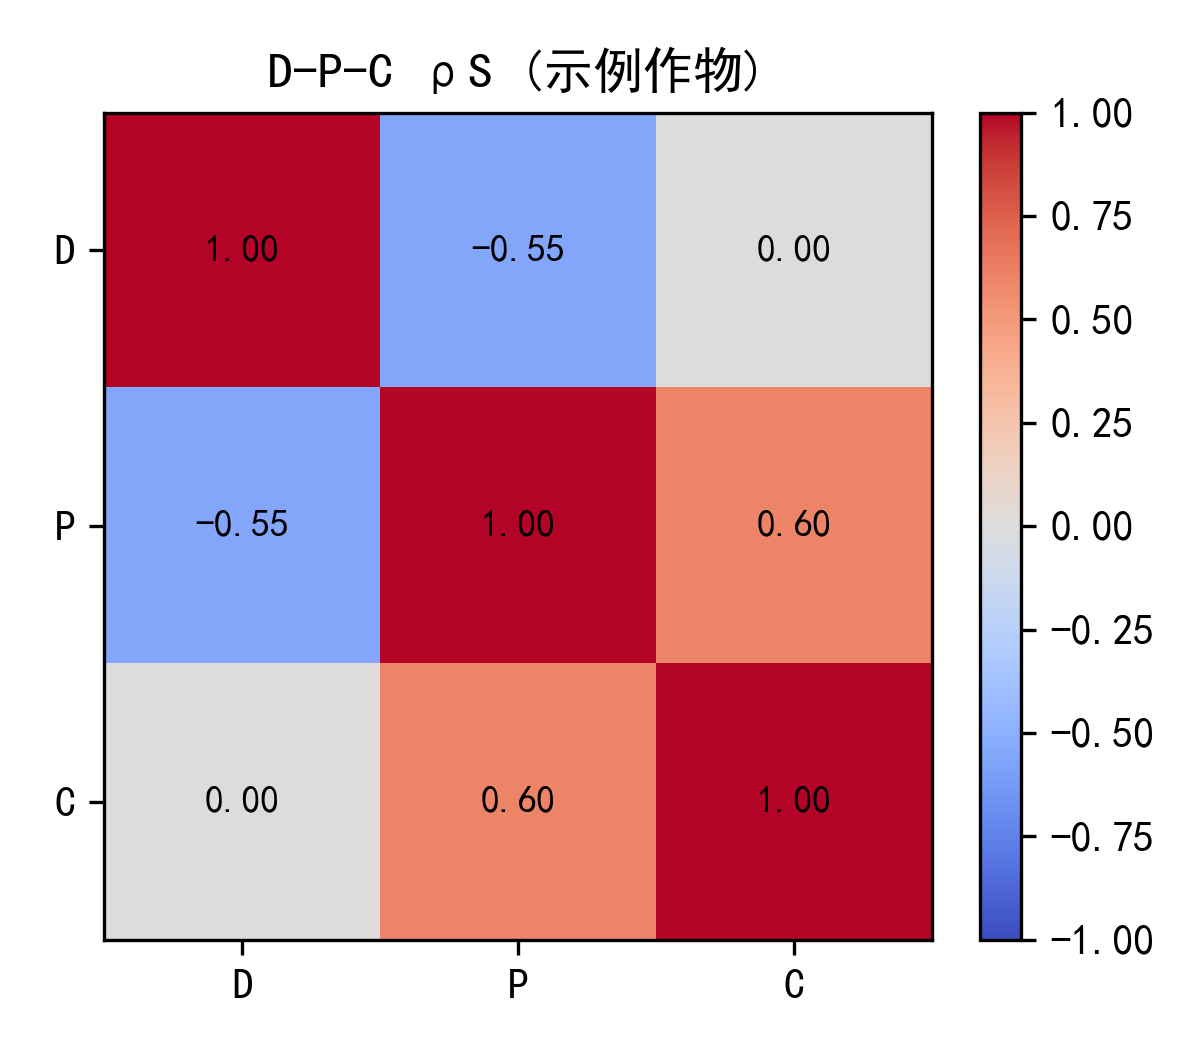
\includegraphics[width=0.85\linewidth]{figure_pb3/triple_block.png}
  \caption{示例作物的 D--P--C 相关性块}
  \label{fig:triple_block}
\end{figure}

\subsection{6.3.2 Copula 检验}
为了检验 Copula 生成的相关性结构是否符合预期，对生成的价格秩与需求秩进行了散点绘制（图~\ref{fig:copula_scatter}）。可以看到，点云呈现一定的负相关趋势（右上稀疏、左上密集），符合价格上升、需求下降的经济逻辑，且分布形态允许非线性关系。

\begin{figure}[htbp]
  \centering
  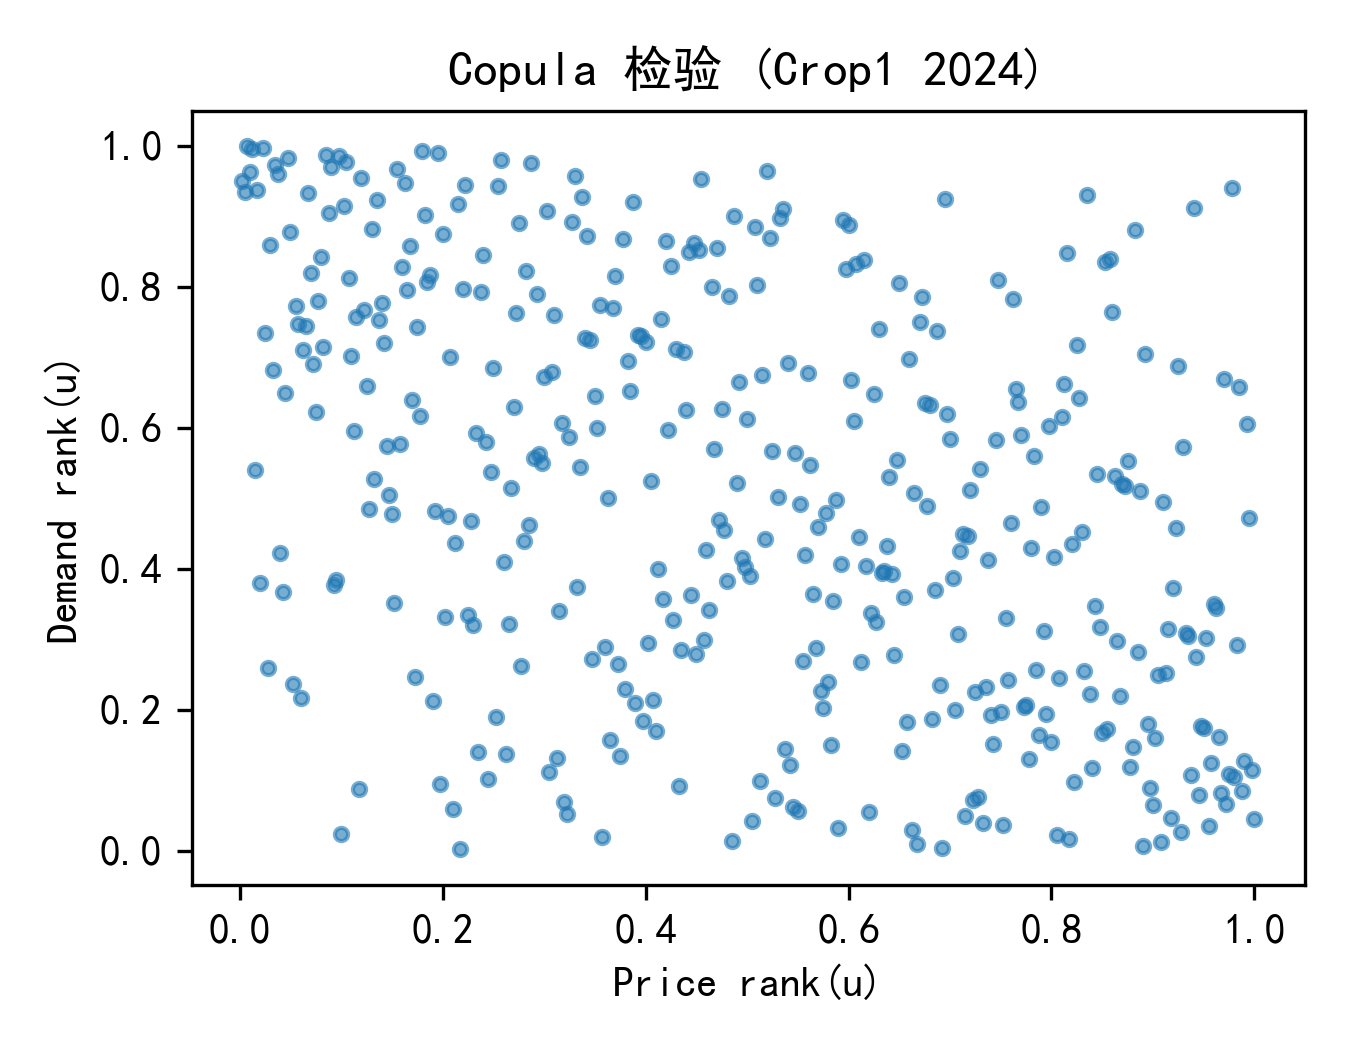
\includegraphics[width=0.78\linewidth]{figure_pb3/666.png}
  \caption{Copula 检验：价格秩 vs 需求秩（Crop1, 2024）}
  \label{fig:copula_scatter}
\end{figure}

\subsection{6.3.3 引入替代性与互补性}
在 Copula 随机场景下，通过交叉价格弹性系数 $\varepsilon_{ij}$ 修正各作物的需求：
\[
D^{\mathrm{adj}}_i = D_i\left(1 + \sum_j \varepsilon_{ij} \cdot \Delta p_j \right), \quad \Delta p_j = \frac{P_j - P_j^{(0)}}{P_j^{(0)}}
\]
其中 $\varepsilon_{ij} > 0$ 表示替代效应（作物 $j$ 涨价将提升 $i$ 的需求），$\varepsilon_{ij} < 0$ 表示互补效应（$j$ 涨价将降低 $i$ 的需求）。

\subsection{6.3.4 风险--收益权衡分析}
采用与问题二相同的目标函数：
\[
\max \; \mathbb{E}[\Pi] - \lambda \cdot \mathrm{CVaR}_{95\%}(\text{亏损})
\]
在不同风险权重 $\lambda$ 下运行 GA 得到的风险--收益前沿如图~\ref{fig:risk_return} 所示。随着 $\lambda$ 增大（风险厌恶程度提高），CVaR95\% 明显降低，极端亏损风险得到有效控制, 期望利润随之下降，呈现出典型的风险--收益权衡关系.$\lambda$ 在 $0.1$ 到 $0.15$ 区间时，利润损失相对有限，但风险降低显著，适合风险偏好中等的决策者。

\begin{figure}[htbp]
  \centering
  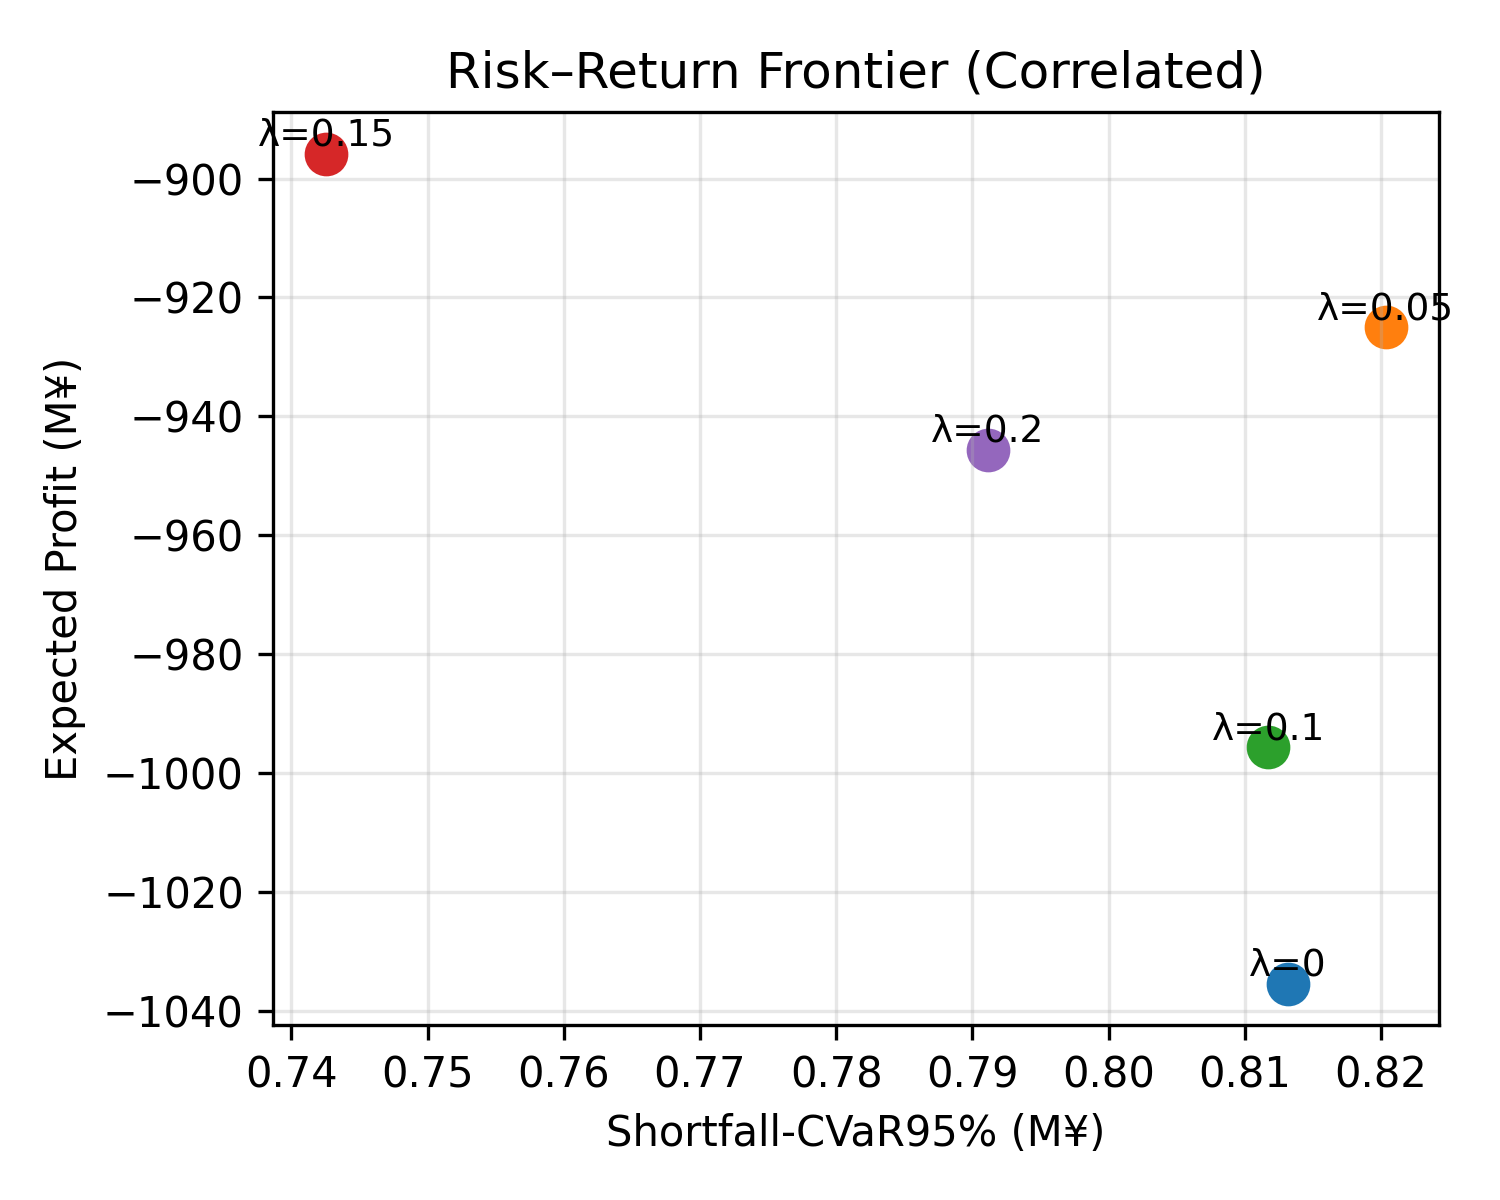
\includegraphics[width=0.82\linewidth]{figure_pb3/34f1e36d36fcf15b8c48d02c32728306.png}
  \caption{风险--收益前沿（含相关性情景）}
  \label{fig:risk_return}
\end{figure}


